\documentclass[tikz]{standalone}

\usepackage[latin1]{inputenc}
\usepackage{tikz}

% GNUPL
\begin{document}

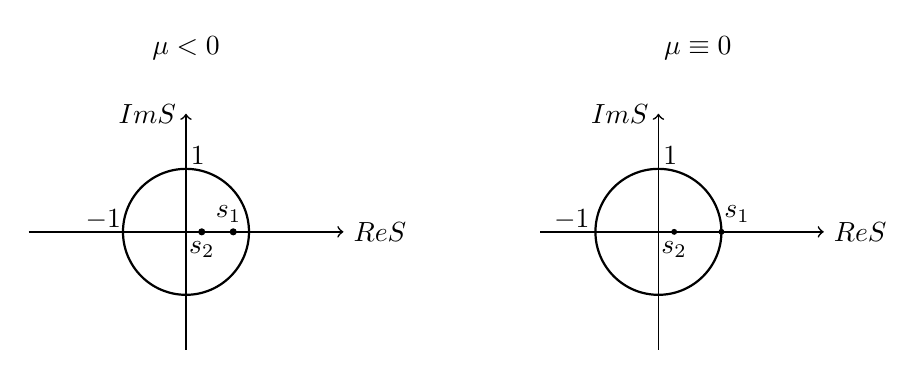
\begin{tikzpicture}
    %\mu<0
    \coordinate [label=-90:$\mu<0$] (8) at (2.5,8.6);
    \draw[semithick] [->] (0.5,6) -- (4.5,6) node[right] {$Re{S}$};
    \draw[semithick] [->] (2.5,4.5) -- (2.5,7.5) node[left] {$Im{S}$};
    \draw[thick] (2.5,6) circle [radius=0.8];
    \coordinate [label=-90:$1$] (8) at (2.65,7.2);
    \coordinate [label=-90:$-1$] (8) at (1.45,6.4);
    \draw[thick] (2.7,6) circle [radius=0.03];
    \draw[thick] (3.1,6) circle [radius=0.03];
    \coordinate [label=-90:$s_2$] (8) at (2.7,6);
    \coordinate [label=90:$s_1$] (8) at (3.04,6);
	%\mu=0
    \coordinate [label=-90:$\mu \equiv0$] (8) at (9,8.6);
    \draw[semithick] [->] (7,6) -- (10.6,6) node[right] {$Re{S}$};
    \draw[semithick] [->] (8.5,4.5) -- (8.5,7.5) node[left] {$Im{S}$};
    \draw [fill] (8.7,6) circle [radius=0.03];
    \draw [fill] (9.3,6) circle [radius=0.03];
    \draw[thick] (8.5,6) circle [radius=0.8];
    \coordinate [label=-90:$1$] (8) at (8.65,7.2);
    \coordinate [label=-90:$-1$] (8) at (7.4,6.4);
    \coordinate [label=-90:$s_2$] (8) at (8.7,6);
    \coordinate [label=90:$s_1$] (8) at (9.5,6);
\end{tikzpicture}


\end{document}